\documentclass[UTF8,a4paper,14pt]{ctexart}
\usepackage[utf8]{inputenc}
\usepackage{amsmath}
\usepackage{amssymb}
\usepackage{amsfonts}
%for 字體
%https://tug.org/FontCatalogue/
% \usepackage[T1]{fontenc}
% \usepackage{tgbonum}
\usepackage[bitstream-charter]{mathdesign}
\usepackage[T1]{fontenc}
%\usepackage{bm}#粗體
%\usepackage{boondox-calo}
\usepackage{textcomp}
\usepackage{fancyhdr}%导入fancyhdr包
\usepackage{ctex}%导入ctex包
\usepackage{enumitem} %for在Latex使用條列式清單
\usepackage{varwidth}
\usepackage{soul} %for \ul
\usepackage{comment}%\begin{comment}\end{comment}
\usepackage{cancel}%\cancel{}
%\usepackage{unicode-math}
\usepackage{physics}% for derivative/partial derivative

\usepackage[dvipsnames, svgnames, x_11names]{xcolor}

\usepackage[low-sup]{subdepth}
\usepackage{subdepth}

\newcommand{\indep}{\perp \!\!\! \perp}

\usepackage{amsthm}

\usepackage{graphicx}
\graphicspath{ {./images/} }


% \DeclareMathOperator{\E}{\mathbb{E}}
\newcommand{\E}{{\rm I\kern-.3em E}}
\newcommand{\Var}{\mathrm{Var}}
\newcommand{\Cov}{\mathrm{Cov}}
\newcommand{\Corr}{\mathrm{Corr}}
% \DeclareMathOperator{\Var}{\textbf{Var}}
% \DeclareMathOperator{\Cov}{\textbf{Cov}}
% \DeclareMathOperator{\Corr}{\textbf{Corr}}


\DeclareMathSizes{10}{10}{7}{5}

\usepackage[a4paper, margin=1.5in]{geometry}

\usepackage{array, makecell} %


%中英文設定
%\usepackage{fontspec}
% \setmainfont{Computer Modern Sans Serif}
% \setmainfont{TeX Gyre Termes}
% \usepackage{xeCJK} %引用中文字的指令集
%\setCJKmainfont{PMingLiU}
% \setCJKmainfont{DFKai-SB}
% \setmainfont{Times New Roman}
% \setCJKmonofont{DFKai-SB}
\pagenumbering{arabic}%设置页码格式
\pagestyle{fancy}
\fancyhead{} % 初始化页眉
\fancyhead[C]{TSA\quad HW 04\quad  R10A21126\quad  WANG YIFAN\quad   \today}
%\fancyhead[LE]{\textsl{\rightmark}}
%\fancyfoot{} % 初始化页脚
%\fancyfoot[LO]{奇数页左页脚}
%\fancyfoot[LE]{偶数页左页脚}
%\fancyfoot[RO]{奇数页右页脚}
%\fancyfoot[RE]{偶数页右页脚}

% \title{{Econometrics HW 03}}
% \author{R10A21126}
% \date{\today}

%\fancyhf{}
\usepackage{lastpage}
\cfoot{Page \thepage \hspace{1pt} of\, \pageref{LastPage}}

\renewcommand{\headrulewidth}{0.1pt}%分隔线宽度4磅
%\renewcommand{\footrulewidth}{4pt}

\allowdisplaybreaks
\usepackage[english]{babel}
%\usepackage{amsthm}
\newtheorem{theorem}{Theorem}[section]
\newtheorem{corollary}{Corollary}[theorem]
\newtheorem{lemma}[theorem]{Lemma}


\usepackage[most]{tcolorbox}
% \newtcbtheorem{Problem}{\bfseries Problem}{enhanced,arc= 1 mm,boxrule=0pt,frame hidden,
%   colback = Pink!50!White,
%   coltitle=black,
%   top=0.15in,
%   attach boxed title to top left=
%   {xshift=1.5em,yshift=-\tcboxedtitleheight/2},
%   boxed title style={size=small,colback=LightPink!70!White}
% }{}
\definecolor{babyblue}{rgb}{0.54, 0.81, 0.94}

\newtcolorbox[auto counter]{mybox}[1]{
    enhanced,
    arc= 1 mm,boxrule=1pt,
    colframe=pink!90!white,
    colback=white,
    coltitle=black,
    % colback=blue!5!white,
    attach boxed title to top left=
    {xshift=1.5em,yshift=-\tcboxedtitleheight/2},
    boxed title style={size=small,
    % frame hidden,
    colback=LightPink!10!White},
    top=0.15in,
    % fonttitle=\bfseries,
    title= {#1},
    subtitle style={boxrule=0.4pt,
              colback=yellow!10!red!10!white},
    breakable
  }
\newtcolorbox[auto counter]{Problem}[1]{
    enhanced,drop shadow={blue!5!white},
    colframe=babyblue!50!,
    fonttitle=\bfseries,
    title=Problem ~\thetcbcounter. #1,
    %separator sign={.},
    coltitle=black,
    colback=blue!3,
    top=0.15in,
    breakable
  }

\newenvironment{solution}
  {\renewcommand\qedsymbol{$\blacksquare$}\begin{proof}[Solution]}
  {\end{proof}}

\theoremstyle{definition}
\newtheorem{definition}{Definition}[section]

%\theoremstyle{notation}
\newtheorem*{notation}{\underline{Notation}}
%\newtheorem*{convention}{\underline{Convention}}
\newtheorem*{convention}{\underline{Convention}}

\theoremstyle{remark}
\newtheorem*{remark}{Remark}

\newenvironment{amatrix}[2]{%% [2] for 2 parameters 
  \left[\begin{array}
    %{cc|cc}
    %  {@{}*{#2}{c}|c*{#1}{c}}
     {{}*{#1}{c}|c*{#2}{c}}
}{%
  \end{array}\right]
}
% For augmented matrix  
%https://tex.stackexchange.com/questions/2233/whats-the-best-way-make-an-augmented-coefficient-matrix



\usepackage{pgfplots}
\pgfplotsset{width=10cm,compat=1.18}
% \pgfplotsset{width=10cm,compat=0.9}
\usepackage{csvsimple}
\usepackage{enumitem}


\begin{document}

\begin{Problem}{}
  The two time series plots are shown below. For each of the series, describe the sample autocorrelations
  \(\hat{\rho}_1\) and \(\hat{\rho}_2\) using the terms strongly positive, moderately positive, near zero, moderately negative, or strongly negative. Do you need to know the scale of measurement for the series to answer?
  
\end{Problem}

\centering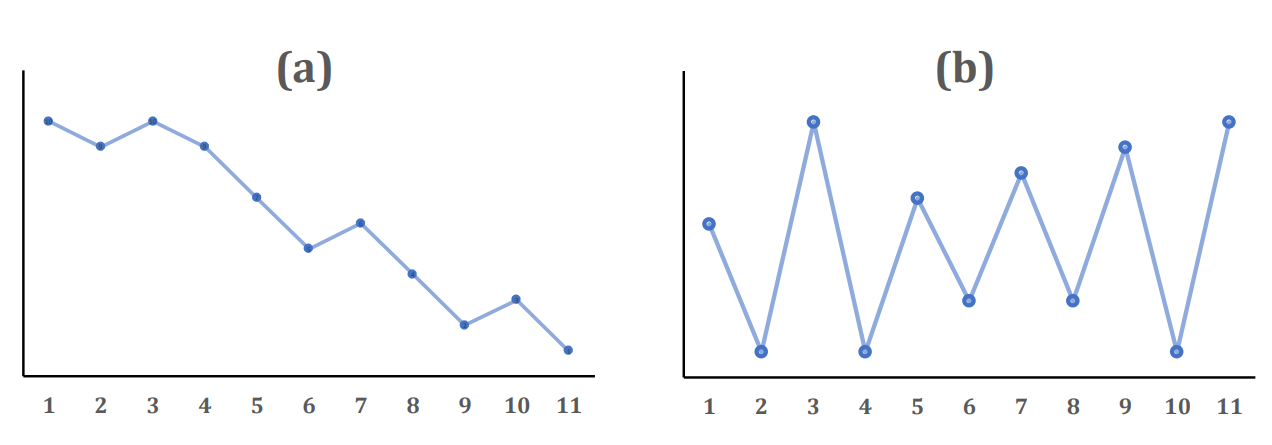
\includegraphics[height=3.5cm]{Q1}

\begin{solution}\,\\
  The scale of measurement is not needed to describe the autocorrelations.

  \begin{mybox}{(a)}
    
    \tcbsubtitle{\(\hat{\rho}_1\)} 
    
      moderately positive  

      The neighboring values are in general on the same side of the mean but in a decreasing trend with fluctuation.
    \tcbsubtitle{\(\hat{\rho}_2\)}   

    moderately positive  

    The alternationing values are in general on the same side of the mean but in a decreasing trend with fluctuation.
  \end{mybox}
  \begin{mybox}{(b)}
    
    \tcbsubtitle{\(\hat{\rho}_1\)} 

    moderately negative

    The neighboring values are always on the different sides of the mean with similar (not always the same) distances.
    \tcbsubtitle{\(\hat{\rho}_2\)} 

    moderately positive  

    The alternationing values are always on the same side of the mean with similar (not always the same) distances.  
  \end{mybox}
\end{solution}

\pagebreak
\begin{Problem}{}
  Identify the \((p, d, q)\) for following ARIMA models and calculate the \(\E[\nabla y_t]\) and \(\Var[\nabla y_t]\).
  \begin{enumerate}[label=(\alph*), ref=\alph*]
    \item \(y_t = 3+y_{t-1}+a_t-0.75a_{t-1}\)
    \item \(y_t = 10+1.25y_{t-1}-0.25y_{t-2}+a_t-0.1a_{t-1}\)
    \item \(y_t = 5+2y_{t-1}-1.7y_{t-2}+0.7y_{t-3}+a_t-0.5 a_{t-1}+0.25 a_{t-2}\)
  \end{enumerate}
\end{Problem}
\begin{solution}\,\\

  \begin{mybox}{(a) \(y_t = 3+y_{t-1}+a_t-0.75a_{t-1}\)}
    \begin{equation*}
      \begin{aligned}
        \nabla y_t 
        &= y_t-y_{t-1}\\
        &=3+a_t-0.75a_{t-1}
      \end{aligned}
    \end{equation*}
    So the model is a stationary, invertible, IMA(1,1) model with \( \theta_1 = 0.75\), and \(L=3\)


    \tcbsubtitle{\(\E[\nabla y_t ]\)}  
    \begin{equation*}
      \begin{aligned}
        \E[\nabla y_t] 
        &=\E[3+a_t-0.75a_{t-1}]\\
        &=3
      \end{aligned}
    \end{equation*}   
     \tcbsubtitle{\(\Var[\nabla y_t ]\)}  
    \begin{equation*}
      \begin{aligned}
        \Var[\nabla y_t ]
        &=\Var[3+a_t-0.75a_{t-1}]\\
        &=[1+0.75^2]\sigma_{a}^2
      \end{aligned}
    \end{equation*}
    

  \end{mybox}



  \begin{mybox}{(b)\(y_t = 10+1.25y_{t-1}-0.25y_{t-2}+a_t-0.1a_{t-1}\)}
    \begin{equation*}
      \begin{aligned}
        \nabla y_t 
        &= y_t-y_{t-1}\\
        &=10+0.25y_{t-1}-0.25y_{t-2}+a_t-0.1a_{t-1}\\
        \nabla y_t -0.25\nabla y_{t-1}&=10+a_t-0.1a_{t-1}
      \end{aligned}
    \end{equation*}
    So the model is a stationary, invertible, ARIMA(1,1,1) model with 
        \begin{equation*}
      \begin{aligned}
        \phi &= 0.25\\
        \theta &= 0.1\\
        L &= 10
      \end{aligned}
    \end{equation*}
    \begin{equation*}
      \begin{aligned}
        \nabla y_t 
        &= y_t-y_{t-1}\\
        &=10+0.25y_{t-1}-0.25y_{t-2}+a_t-0.1a_{t-1}\\
        &=10+0.25 \nabla y_{t-1}+a_t-0.1a_{t-1}\\
        &=10+0.25 (10+0.25 \nabla y_{t-2}+a_{t-1}-0.1a_{t-2})+a_t-0.1a_{t-1}\\
        &=\cdots
      \end{aligned}
    \end{equation*}



    \tcbsubtitle{\(\E[\nabla y_t ]\)} 
    
    \begin{equation*}
      \begin{aligned}
        \E[\nabla y_t ]
        &= \E[10+0.25(10+0.25\nabla y_{t-1})]\\
        &= \E[10+0.25(10)+(0.25)^2(10+0.25\nabla y_{t-2})]\\
        &= \E[10+0.25(10)+(0.25)^2(10)+(0.25)^3(10)+\cdots]\\
        &=\frac{10}{1-0.25}\\
        &=\frac{40}{3}
      \end{aligned}
    \end{equation*}
    
    \tcbsubtitle{\(\Var[\nabla y_t ]\)}         
    \begin{equation*}
      \begin{aligned}
        \Var[\nabla y_t ]
        &= \frac{1-2\phi\theta+\theta^2}{1-\phi^2}\sigma_a^2\\
        &= \frac{1-2(0.25)(0.1)+(0.1)^2}{1-(0.25)^2}\sigma_a^2\\
        &=1.024\sigma_a^2
      \end{aligned}
    \end{equation*}
  \end{mybox}


  \begin{mybox}{(c)\(y_t = 5+2y_{t-1}-1.7y_{t-2}+0.7y_{t-3}+a_t-0.5 a_{t-1}+0.25 a_{t-2}\)}
    \begin{equation*}
      \begin{aligned}
        \nabla y_t 
        &= y_t-y_{t-1}\\
        &=5+y_{t-1}-1.7y_{t-2}+0.7y_{t-3}+a_t-0.5 a_{t-1}+0.25 a_{t-2}\\
        &=5+y_{t-1}-y_{t-2}-0.7y_{t-2}+0.7y_{t-3}+a_t-0.5 a_{t-1}+0.25 a_{t-2}\\
        &=5+\nabla y_{t-1}-0.7\nabla y_{t-2}+a_t-0.5 a_{t-1}+0.25 a_{t-2}\\
      \end{aligned}
    \end{equation*}
    Thus we have
    \begin{equation*}
      \begin{aligned}
        \nabla y_t -\nabla y_{t-1}+0.7\nabla y_{t-2}
        &=5+a_t-0.5a_{t-1}+0.25 a_{t-2}\\
        (1-B+0.7B^2)\nabla y_t &= 5+(1-0.5B+0.25B^2)a_t
      \end{aligned}
    \end{equation*}
    For the AR(2) part, we have
    \begin{equation*}
      \begin{aligned}
      \phi_1 &= 1\\
      \phi_2 &= -0.7
      \end{aligned}
    \end{equation*}
    Stationarity conditions for the ARMA(2)
    model:    \begin{equation}
      \begin{aligned}\label{eq:4.3.11}
      \phi_1 + \phi_2 &<1\\
      \phi_2 - \phi_1 &<1\\
      \left\lvert \phi_2\right\rvert  &< 1
      \end{aligned}
    \end{equation}
    
    Check the stationarity conditions
    \begin{equation*}
      \begin{aligned}
      (1) + (-0.7) &<1\\
      (-0.7) - (1) &<1\\
      \left\lvert -0.7\right\rvert  &< 1
      \end{aligned}
    \end{equation*}


    So the model is a stationary ARIMA(2,1,2) model


    \tcbsubtitle{\(\E[\nabla y_t ]\)} 
    \begin{equation*}
      \begin{aligned}
        \E[\nabla y_t] 
        &=\E[5+\nabla y_{t-1}-0.7\nabla y_{t-2}+a_t-0.5 a_{t-1}+0.25 a_{t-2}]\\
        &=5+\E[\nabla y_{t-1}]-0.7\E[\nabla y_{t-2}]\\
      \end{aligned}
    \end{equation*}
    Due to stationarity,  \(\E[\nabla y_t]\) is a constant for all \(t\). Thus we have
    \begin{equation*}
      \begin{aligned}
        \E[\nabla y_t] 
        &=5+\E[\nabla y_{t}]-0.7\E[\nabla y_{t}]\\
        % 0.7\E[\nabla y_{t}]
        % &=5\\
        \E[\nabla y_{t}]
        &=\frac{5}{0.7}\\
        &=\frac{50}{7} = \mu_w
      \end{aligned}
    \end{equation*}

    
    
    \tcbsubtitle{\(\Var[\nabla y_t ]\)}  


    Let
    \begin{equation*}
      \begin{aligned}
        w_t = \nabla y_t
      \end{aligned}
    \end{equation*}
    \begin{equation*}
      \begin{aligned}
        \tilde{w}_t &= w_t-\mu_w
        &= \nabla y_t -\mu_w
      \end{aligned}
    \end{equation*}
    Thus we have \(\E[\tilde{w}_t]=0\) and
    \begin{equation*}
      \begin{aligned}
        \phi(B)\tilde{w}_t &= w_t-\mu_w\\
        &= \nabla y_t -\mu_w=\theta(B)a_t
      \end{aligned}
    \end{equation*}

    For \(\tilde{w}_t\), the moving average representation
    \begin{equation}\
      \begin{aligned}
        \tilde{w}_t = \psi(B)a_t =\sum_{j = 0}^{\infty} \psi_j a_{t-j} 
      \end{aligned}
    \end{equation}
    where
      \begin{equation}\
        \begin{aligned}
        \psi(B) = \frac{\theta(B)}{\phi(B)}
        \end{aligned}
      \end{equation}
      The weights \(\psi\) are determined from the relation \(\psi(B) \phi(B)= \theta(B)\) to satisfy
      \begin{equation}\
        \begin{aligned}
        \psi_j = \phi_1\psi_{j-1}+\phi_2\psi_{j-2}+\cdots+\phi_p\psi_{j-p}-\theta_j\quad j>0
        \end{aligned}
      \end{equation}
      with \(\psi_0 = 1, \psi_j = 0\) for \(j<0\), and \(\theta_j = 0\) for \(j>q\)
      \begin{equation*}\
        \begin{aligned}
        \psi_0 &= 1\\
        \psi_1 &= \phi_1\psi_0+\phi_2\psi_{-1}-\theta_1\\
        &=(1)(1)+(-0.7)(0)-(0.5)\\
        &=0.5\\
        \psi_2 &= \phi_1\psi_1+\phi_2\psi_{0}-\theta_2\\
        &=(1)(0.5)+(-0.7)(1)-(-0.25)\\
        &=0.05
      \end{aligned}
      \end{equation*}

      The autocovariance function may be expressed as
      \begin{equation}
        \begin{aligned}\label{eq:3.4.2}
          \gamma_k &= \phi_1\gamma_{k-1}+\cdots+\phi_p\gamma_p-\sigma_a^2(\theta_k\psi_0+\theta_{k+1}\psi_1+\cdots+\theta_p\psi_{q-k})\\
        \end{aligned}
      \end{equation}
      with the convention that \(\theta_0 = -1\).

      For \(k = 0,1,2\)

      \begin{equation*}
        \begin{aligned}
          \gamma_0 &= \phi_1\gamma_1+\phi_2\gamma_2-\sigma_a^2(\theta_0\psi_0+\theta_1\psi_1+\theta_2\psi_2)\\
          \gamma_1 &= \phi_1\gamma_0+\phi_2\gamma_1-\sigma_a^2(\theta_1\psi_0+\theta_2\psi_1)\\
          \gamma_2 &= \phi_1\gamma_1+\phi_2\gamma_0-\sigma_a^2(\theta_2\psi_0)
        \end{aligned}
      \end{equation*}


      \begin{equation*}
        \begin{aligned}
          \gamma_0 &= (1)\gamma_1+(-0.7)\gamma_2-\sigma_a^2(-1+(0.5)(0.5)+(-0.25)(0.05))\\
          \gamma_1 &= (1)\gamma_0+(-0.7)\gamma_1-\sigma_a^2((0.5)(1)+(-0.25)(0.5))\\
          \gamma_2 &= (1)\gamma_1+(-0.7)\gamma_0-\sigma_a^2((-0.25)(1))
        \end{aligned}
      \end{equation*}
      \begin{equation*}
        \begin{aligned}
          \gamma_0 &= \gamma_1+(-0.7)\gamma_2-\sigma_a^2(-0.7625)\\
          \gamma_1 &= \gamma_0+(-0.7)\gamma_1-\sigma_a^2(0.375)\\
          \gamma_2 &= \gamma_1+(-0.7)\gamma_0-\sigma_a^2(-0.25)
        \end{aligned}
      \end{equation*}
      Solving the equations, the variance\(\gamma_0\) of the process \({\tilde{w}_t}\) is obtained as
      \begin{equation*}
          \gamma_0 \approx 1.563\sigma_a^2
      \end{equation*}

      For \(w_t = \nabla y_t\)

      \begin{equation*}
        \begin{aligned}
          \gamma_0(w_t) = \Var[w_t]
          &= \Var[{\tilde{w}_t}+\mu_w]
          = \Var[{\tilde{w}_t}]=\gamma_0({\tilde{w}_t})
          &\approx 1.563\sigma_a^2
        \end{aligned}
      \end{equation*}      
      % \begin{equation*}
      %   \begin{aligned}
      %     \gamma_k &= \E[w_t w_{t-k}]-\E[w_t]\E[w_{t-k}]\\
      %     &=\E[(5+w_{t-1}-0.7w_{t-2}+a_t-0.5 a_{t-1}+0.25 a_{t-2})w_{t-k}]-\E[w_t]\E[w_t]\\
      %     &=5\E[w_{t-k}]+\E[w_{t-1} w_{t-k}]-0.7\E[w_{t-2}w_{t-k}]\\
      %     &\,\,+\E[a_t w_{t-k}]-0.5\E[a_{t-1} w_{t-k}]+0.25\E[a_{t-2} w_{t-k}]-\E[w_t]\E[w_t]\\
      %     &=(\E[w_{t-1} w_{t-k}]-\E[w_{t-1}]\E[w_{t-k}])-0.7(\E[w_{t-2}w_{t-k}]-\E[w_{t-2}]\E[w_{t-k}])\\
      %     &\,\,+\E[a_t w_{t-k}]-0.5\E[a_{t-1} w_{t-k}]+0.25\E[a_{t-2} w_{t-k}]+5\E[w_t]-\E[w_t]\E[w_t]+\E[w_t]\E[w_t]-0.7\E[w_t]\E[w_t]\\
      %     &=\gamma_{k-1} -0.7\gamma_{k-2}+\gamma_{wa}(k)-0.5\gamma_{wa}(k-1)+0.25\gamma_{wa}(k-2) +5\E[w_t]-0.7\E[w_t]\E[w_t]\\
      %   \end{aligned}
      % \end{equation*}
      % where \(\gamma_{wa}(k)\) is the cross-covariance function between \(w\) and \(a\) and is defined by \(\gamma_{wa}(k) = \E[w_{t-k}a_t]\)
  \end{mybox}
\end{solution}

\pagebreak
\begin{Problem}{}
  Suppose that \(y_t = A+Bt+x_t\), where \(x_t\)
  is a random walk. First suppose that A and B are constants.
  \begin{enumerate}[label=(\alph*), ref=\alph*]
    \item Is \(y_t\) stationary?
    \item Is \(\nabla y_t\) stationary?
  \end{enumerate}
  Now let \(A\) and \(B\) be random variables that are independent of the random walk \(x_t\).
  \begin{enumerate}[label=(\alph*), ref=\alph*]\setcounter{enumi}{2}
    \item Is \(y_t\) stationary?
    \item Is \(\nabla y_t\) stationary?
  \end{enumerate}

\end{Problem}


\begin{solution}
  \,
  \begin{mybox}{(a)}
    \begin{equation*}
      \begin{aligned}
        \E[y_t] 
        &=\E[A+Bt+x_t]\\
        &=A+Bt
      \end{aligned}
    \end{equation*}
    which depends on \(t\). So \(y_t\) is not stationary.
  \end{mybox}

  \begin{mybox}{(b)}
    \begin{equation*}
      \begin{aligned}
        \nabla y_t
        &=y_t - y_{t-1}\\
        &=A+Bt+x_t - (A+B(t-1)+x_{t-1})\\
        &=B+x_t-x_{t-1}
      \end{aligned}
    \end{equation*}
    \begin{equation*}
      \begin{aligned}
        \E[\nabla y_t] 
        &=\E[B+x_t-x_{t-1}]\\
        &=B
      \end{aligned}
    \end{equation*}
    which is a constant.
    \begin{equation*}
      \begin{aligned}
        \Cov[\nabla y_t,\nabla y_{t-k}] 
        &=\Cov[B+x_t-x_{t-1},B+x_{t-k}-x_{t-k-1}]\\
        &=\Cov[x_t-x_{t-1},x_{t-k}-x_{t-k-1}]\\
        &=\Cov[x_t,x_{t-k}]
        +\Cov[x_t,-x_{t-k-1}]\\
        &\,\,+\Cov[-x_{t-1},x_{t-k}]
        +\Cov[-x_{t-1},-x_{t-k-1}]\\
        &=\begin{cases}
          2\sigma_a^2 & k=0\\
          -\sigma_a^2 & k=1\\
          0 &k>1
        \end{cases}
      \end{aligned}
    \end{equation*}
    which does not depend on \(t\). 
    
    
    So \(\nabla y_t\) is stationary.
  \end{mybox}

  \begin{mybox}{(c)}
    \begin{equation*}
      \begin{aligned}
        \E[y_t] 
        &=\E[A+Bt+x_t]\\
        &=\E[A]+\E[B]t
      \end{aligned}
    \end{equation*}
    which depends on \(t\). So \(y_t\) is not stationary.
  \end{mybox}
  \begin{mybox}{(d)}
    \begin{equation*}
      \begin{aligned}
        \nabla y_t
        &=y_t - y_{t-1}\\
        &=A+Bt+x_t - (A+B(t-1)+x_{t-1})\\
        &=B+x_t-x_{t-1}
      \end{aligned}
    \end{equation*}
    \begin{equation*}
      \begin{aligned}
        \E[\nabla y_t] 
        &=\E[B+x_t-x_{t-1}]\\
        &=\E[B]
      \end{aligned}
    \end{equation*}
    which is a constant.
    \begin{equation*}
      \begin{aligned}
        \Cov[\nabla y_t,\nabla y_{t-k}] 
        &=\Cov[B+x_t-x_{t-1},B+x_{t-k}-x_{t-k-1}]\\
        &=\Cov[B,B]\\
        &\,\,+\Cov[x_t,x_{t-k}]
        +\Cov[x_t,-x_{t-k-1}]\\
        &\,\,+\Cov[-x_{t-1},x_{t-k}]
        +\Cov[-x_{t-1},-x_{t-k-1}]\\
        &=\begin{cases}
          \Var[B]+2\sigma_a^2 & k=0\\
          \Var[B]+(-\sigma_a^2) & k=1\\
          \Var[B] &k>1
        \end{cases}
      \end{aligned}
    \end{equation*}
    which does not depend on \(t\). 
    
    
    So \(\nabla y_t\) is stationary.
  \end{mybox}
\end{solution}

\pagebreak
\begin{Problem}{}
  Given a stationary process \(y_t\), show that if \(\rho_1 < 0.5\), \(\nabla y_t\) has a larger variance than does \(y_t\)
\end{Problem}

\begin{solution}
  \begin{equation}\
    \begin{aligned}
      \Var[\nabla y_t]
     &= \Var[(1-B)y_{t}] \\
     &= \Var[y_{t}-y_{t-1}]\\
     &=\Var[y_{t}]+\Var[y_{t-1}]-2\Cov[y_{t},y_{t-1}]\\
     &=\gamma_0+\gamma_0-2\gamma_1\\
     &=(2-2\rho_1)\gamma_0\\
     &=\underset{>1}{\underbrace{2(1-\rho_1)}}\gamma_0\\
     &>\gamma_0\\
    \end{aligned}
  \end{equation}
  We then conclude that \(\nabla y_t\) has a larger variance than does \(y_t\).
\end{solution}

\end{document}